\section{Experimental Evaluation}
\label{section:evaluation}
Our evaluation of \sawfish includes a comparison with two competitors, and we investigate the scaling behavior of \sawfish.
Finally, we look into the actual dependencies that \sawfish produces, and examine their usefulness. We publicly provide all source code\footnote{\url{https://github.com/HPI-Information-Systems/Sawfish}}.

\subsection{Experimental Setup}
All experiments were run on an Ubuntu-based (20.04 LTS) server, equipped with two Intel Xeon E5-2650 processors and 256~GB of RAM\@.
All algorithms are single-threaded, running on Java~11 and reading their input data from CSV files.
We do not use the entire main memory, but set explicit memory limits for the Java Virtual Machine.
We use a 4~GB limit for all datasets, except for the \emph{IMDB} dataset, which uses 32~GB.
Moreover, we set a time limit of 24~hours, aborting executions that exceeded that time threshold. 
Unless stated otherwise, all experiments were run three times, and we present the mean of the runs.

\sawfish is compatible with the \emph{Metanome} data profiling platform~\cite{papenbrock2015metanome},
which handles both file and database backed inputs and provides a unified view for the algorithms.
We used the \emph{metanome-cli} to conduct the experiments in a repeatable and efficient way. 

We use four publicly available datasets\footnote{\url{https://hpi.de/naumann/projects/repeatability/data-profiling/metanome-ind-algorithms.html}}: three real-world datasets, and the synthetic TPC-H dataset.
Table~\ref{table:eval:datasets} shows the datasets and their characteristics.
The number in parentheses indicates the number of ignored attributes (due to values containing more than 50 characters or more than ten tokens).
The number of distinct values across all columns excludes the values of the ignored columns.
\begin{table}[ht]
\centering
\caption{Summary of datasets used in the experiments.}
\label{table:eval:datasets}
\begin{tabular}{@{}lrrrr@{}}
\toprule
     & size (MB)   & cols (ignored)  & rows   & distincts   \\
\midrule
CENSUS    & \num{112}         & 42 \phantom{1}(0)                & \num{199524}    & \num{101937}            \\
WIKIPEDIA & \num{570}         & 14 \phantom{1}(3)                & \num{14024428}  & \num{6950343}           \\
TPC-H    & \num{1430}        & 61 \phantom{1}(6)                & \num{6001215}   & \num{9547611}           \\
IMDB      & \num{3790}        & 108 (14)              & \num{36244344}  & \num{47539970}          \\
\bottomrule
\end{tabular}
\end{table}



Because there exists no other sIND detection algorithm, we compare \sawfish to a traditional IND detection algorithm and a baseline.
For the former, we choose the state-of-the-art algorithm \algorithmName{Binder}~\cite{papenbrock2015divide} using the authors' implementation.
\algorithmName{Binder} solves a specialized task in comparison to \sawfish, implicitly setting $\tau = 0$. Thus, it can use techniques more tailored to the traditional IND discovery, as we explained in Section~\ref{section:related_work2}.

Also, we compare \sawfish to a baseline solution for each similarity measure -- an approach based on the original string similarity join algorithms \algorithmName{PassJoin}~\cite{PassJoin} and \algorithmName{ScanCount}~\cite{StringSimSurvey}.
Applying the definition of sINDs, we simply similarity-join each value of the dependent column one by one with the referenced column.
If each value of the dependent column finds at least one join partner, the sIND between the dependent and the referenced column holds.
For \algorithmName{PassJoin}, we based our implementation on the \code{EditDistanceJoiner} by the database group of Tsinghua University\footnote{\url{https://github.com/lispc/EditDistanceClusterer}}.
The provided algorithm is capable of handling only strings that are longer than the edit distance threshold.
Therefore, \sawfish also ignores shorter strings when comparing both algorithms.
Since \sawfish can handle strings that are shorter than the edit distance threshold, we process all strings up to length 50 in the other experiments.
Additionally, we implement the commonly known length filter, which compares the minimum and maximum lengths of column pairs.
For \algorithmName{ScanCount}, we did not find a suitable Java implementation, so we implemented a plain Java version ourselves.

\subsection{Runtime Scalability}
This section examines how \sawfish scales in different dimensions.
We investigate the row and column scalability.
Additionally, we analyze the runtime impact of the edit distance threshold.

\subsubsection{Row Scalability}
This experiment investigates the runtime scalability with the number of rows. 
We used random samples: starting with 10\% of the input dataset and then gradually growing the sample size by 10\%.
We repeated this experiment 10 times and plotted the mean and standard deviation.

We present the results for the \emph{CENSUS}, \emph{WIKIPEDIA}, \emph{TPC-H}, and \emph{IMDB}~($JAC$ mode only) datasets in Figure~\ref{fig:eval:row}.
We do not show the \emph{IMDB} dataset in $ED$ mode, as processing the entire dataset exceeds our time limit of 24~hours, as shown in Figure~\ref{fig:eval:comparsion_ed}.
We set the edit distance threshold $\tau=1$ and the Jaccard similarity threshold $\delta = 0.4$.
The solid yellow and blue lines show the runtime of the $JAC$ mode and $ED$ mode, respectively.
The numbers of sINDs are presented as dashed lines in the respective colors.

We observe that \sawfish exhibits a near perfect linear scaling, both in $ED$ mode and $JAC$ mode.
We also observe that the runtime is not dependent on the result set size: in the \emph{CENSUS} and the \emph{WIKIPEDIA} datasets the result set size is almost constant, but the runtime increases similarly to the \emph{TPC-H} and the \emph{IMDB} datasets, where the result set size continuously grows.
However, this independence of runtime and result set size is related to our experimental setup.
\sawfish benefits from discarding sIND candidates early.
Verifying an sIND candidate that is valid is most demanding because, for every dependent value, it probes the index and computes the exact edit distance at least once.
Since we sampled from the input dataset, for all sINDs that do not appear in the result set of smaller data portions, there is a missing value in the referenced column.
The validation effort for other values does not change because we cannot check the dependent value that references the missing value first.
Thus, the validation effort decreases only linearly.
Nonetheless, we can expect \sawfish to scale linearly to even longer datasets.

Interestingly, the variance is higher in $ED$ mode for the \emph{WIKIPEDIA} dataset, while it is higher for the \emph{TPC-H} dataset in $JAC$ mode.
For the \emph{CENSUS} dataset, the overall variance is low due to the short runtime.
The results for the \emph{IMDB} dataset also exhibit little variance and follow the linear trend of the other datasets.
There is even a slight decrease in mean runtime in $JAC$ mode on the \emph{TPC-H} dataset.
However, these longer running samples do not necessarily contain more sINDs.
These artifacts can be linked to the individual dataset characteristics.
If we find dependent values that have many matches in the inverted index, but are in fact dissimilar to all referenced values, the validation takes longer.
By increasing row set sizes, we also increase the number of ``strong'' counterexamples, i.e., counterexamples with no index matches.
We observe a similar behavior in Section~\ref{subsection:similarity_measure_scalability}.


\begin{figure}[ht]
    \centering
    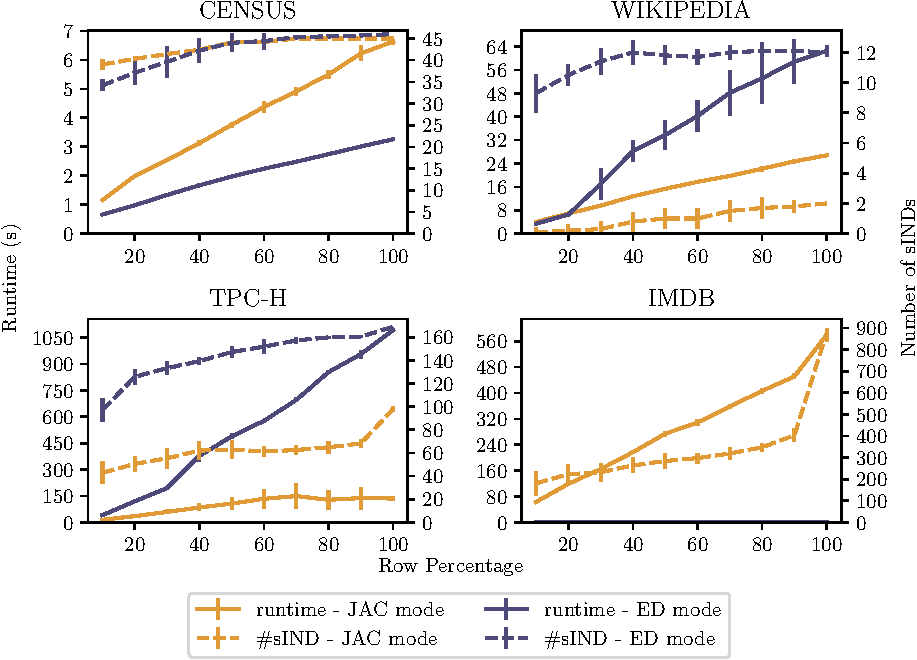
\includegraphics[width=.8\columnwidth]{figures/row_scaling.pdf}
    \caption{Row scalability on different datasets (for $ED$ mode $\tau = 1$, for $JAC$ mode $\delta = 0.4$)}
    \label{fig:eval:row}
\end{figure}

\subsubsection{Column Scalability}
Next, we investigate the scalability of \sawfish with an increasing number of columns.
For this experiment, we randomly sampled column sets for each of the ten column set sizes.
We used 30 samples for each size to accommodate the high variance from different column sets, because the runtime depends on the number of valid sINDs that happen to hold in that sample.
To explain the variance, we take another look at our introductory example, regarding two sets of two columns each.
Let the first set consist of column \mbox{\emph{results[$\mathtt{name}$]}} and column \mbox{\emph{goalie[$\mathtt{p\_id}$]}}, and the second consist of column \emph{results[$\mathtt{name}$]} and column \emph{goalie[$\mathtt{club}$]}.
As the sIND \emph{results[$\mathtt{name}$]~$\simIND{}$~goalie[$\mathtt{club}$]} as well as the symmetric counterpart are valid, \sawfish needs to iterate through both columns, build indices, and validate all dependent values.
On the other hand, we can already determine after preprocessing that there are no sINDs in the first column set, because of their length difference.
Thus, \sawfish can process it much faster.
We investigate the impact of valid dependencies in Section~\ref{subsection:evaluation:valid_impact}.
To emphasize the variance between the results, we present boxplots for each sample size.
Figure~\ref{fig:eval:column_ED} shows the results for the column scalability of the \emph{CENSUS}, \emph{WIKIPEDIA} and \emph{TPC-H} datasets in $ED$ mode.
We omit the \emph{IMDB} dataset for the same reasons as in our row-scaling experiment.

Since the number of sIND candidates grows quadratically in the number of columns, one could expect a quadratic scaling.
However, we observe a linear scaling.
In our experimental setup of sampling from an input dataset, the number of valid sIND candidates on average grows linearly with the number of columns.
Additionally, we find that \sawfish's runtime in general does not grow over-proportionally with rising data amounts.
This shows the effectiveness of \sawfish's memory handling.

While the \emph{CENSUS} dataset shows almost no variance due to its small size, the runtimes vary widely for the \emph{WIKIPEDIA} and the \emph{TPC-H} dataset.
For the \emph{WIKIPEDIA} dataset, we observe a small runtime variance for column sets of sizes 10 and 11, as only a few sets have such column counts.
The remaining variance can be attributed to the differences between the three experiment runs.
However, we observe some outliers.
On the one hand, there are two outliers for column set size 10 that have a drastically reduced runtime.
On the other hand, there are two outliers for column set sizes 3 to 5 that have a drastically increased runtime.
For column set size 2, there are also a few outliers.
These are artifacts related to the difference between processing a valid sIND and quickly discarding an invalid candidate, as we explained before.
However, they are also related to the dataset ``shape''.
The \emph{WIKIPEDIA} dataset consists of two tables:
Table~1 is wider, while Table~2 is longer.
There exists the valid sIND \emph{Table1[$\mathtt{column9}$]} $\simIND{}$ \emph{Table2[$\mathtt{column1}$]}.
It takes roughly 40~seconds to validate this sIND alone, explaining the extreme outlier for column set size~2.
This sIND is also responsible for the two outliers for column set size~10.
There are similar explanations for the other outliers.

When using $JAC$ as similarity measure, the results in Figure~\ref{fig:eval:column_JAC} for the \emph{WIKIPEDIA} dataset look quite similar.
While we can process the data faster overall, the scalability differs not much.
We observe similar outliers because they are not specific to the $ED$ mode.

\begin{figure}
    \centering
    \begin{subfigure}[t]{0.4\textwidth}
        \vskip 0pt
        \centering
        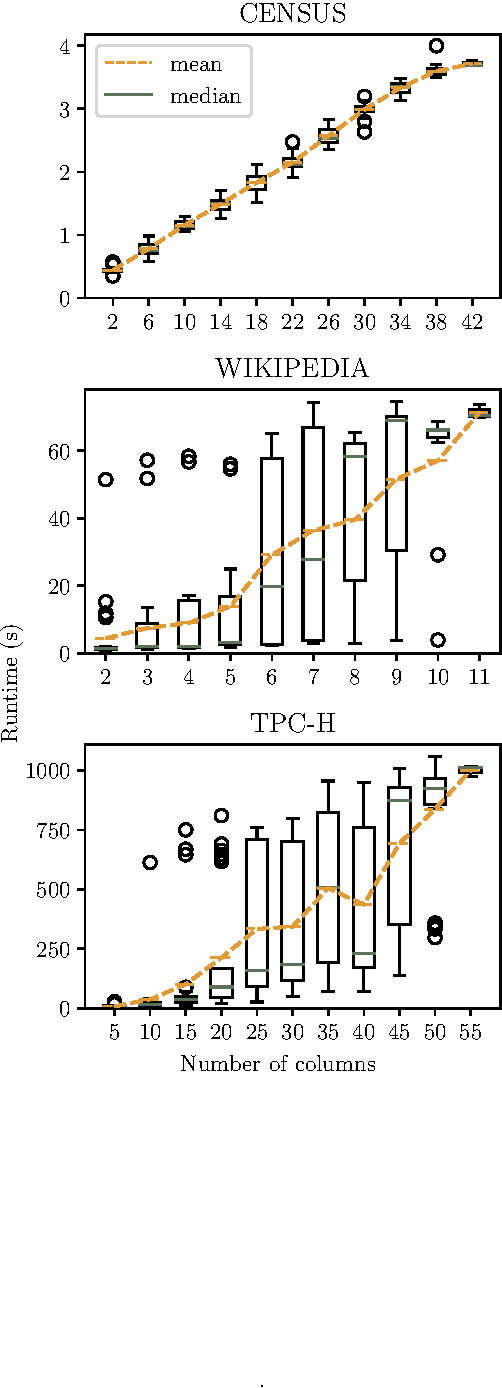
\includegraphics[width=\textwidth]{figures/column_scaling_ed.pdf}
        \caption{$ED$ mode ($\tau = 1$)}
        \label{fig:eval:column_ED}
    \end{subfigure}
    \begin{subfigure}[t]{0.4\textwidth}
        \vskip 0pt
        \centering
        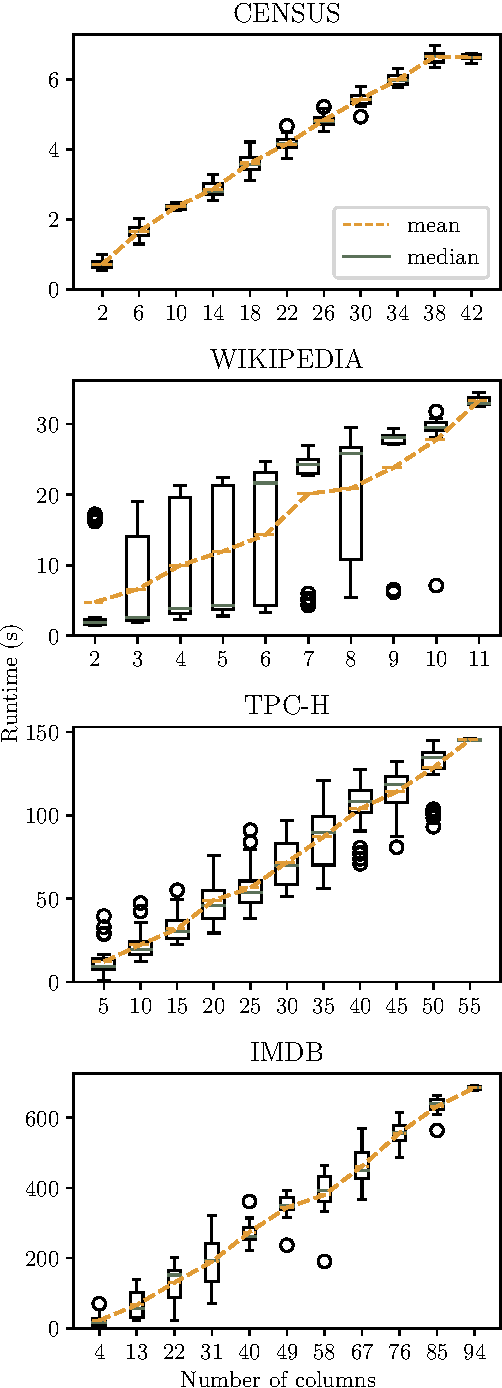
\includegraphics[width=\textwidth]{figures/column_scaling_jac.pdf}
        \caption{$JAC$ mode ($\delta = 0.4$)}
        \label{fig:eval:column_JAC}
    \end{subfigure}
    \caption{Column scalability on different datasets}
    \label{fig:eval:column}
\end{figure}

For the \emph{TPC-H} dataset, \sawfish's column scaling behaves similarly.
Figure~\ref{fig:eval:column} also shows some outliers in $ED$ mode.
However, these exist for the same reasons, as in the \emph{WIKIPEDIA} dataset.
Similarly to the \emph{WIKIPEDIA} dataset, the general scaling seems to be linear as well.
We observe another artifact of our random sampling: the mean runtime for the column set size 40 is in fact lower than the mean runtime for column set size 35.
Due to the large number of possible column sets of these sizes, such a deviation can occur because of the differences in runtime of individual column combinations.
Interestingly, there seems to be a column set of size 50 that takes longer to process than the entire dataset.
The reason for this result is simply normal measuring deviation.

In comparison to the $ED$ mode, the column scalability on the \emph{TPC-H} dataset in Figure~\ref{fig:eval:column_JAC} in $JAC$ mode presents a near perfect linear scaling of the mean runtime.
We still observe outliers, but the overall variance is lower.
Due to the lower overall runtime, the time spent on processing the input has a larger share of the entire runtime.
Because the input handling is less dependent on specific data characteristics, it differs less than the validation time for equal sample sizes.
Even on the largest \emph{IMDB} dataset, the observed column scaling is linear.
We also observe some outliers that are present for similar reasons as in \emph{WIKIPEDIA} and \emph{TPC-H} datasets.
However, the overall variance compared to the absolute runtime is lower.
This experiment shows that \sawfish's column scaling behavior can be replicated on larger datasets.

\subsubsection{Similarity Measure Thresholds}
\label{subsection:similarity_measure_scalability}
This section examines the impact of the only functional configuration parameter: the similarity threshold.
For the $ED$ mode, this is the number of allowed edits $\tau$.
For the $JAC$ mode, this is the similarity threshold $\delta$.

\paragraph{Edit Distance Threshold}
We investigate the edit distance threshold on two datasets:  \emph{CENSUS} and \emph{WIKIPEDIA}.
We run \sawfish with an edit distance threshold $\tau$ between $0$ and $6$.
We choose 6 as the upper bound, because beyond that threshold a majority of the strings consists of less than $\tau$ characters.
We do not evaluate the other datasets, as they cannot be processed for $\tau = 6$ within our time limit of 24~hours.
Figure~\ref{fig:eval:ed} shows the results for the \emph{CENSUS} dataset.
We plot the runtime and the number of valid sINDs.
While the runtime stays almost constant for lower edit distance thresholds, it quickly rises for $\tau \geq 4$.
In contrast, the result set grows over the entire experiment, despite a growing number of simple sINDs (all value lengths are $\leq \tau$).

\begin{figure}
    \centering
    \begin{subfigure}[b]{.8\textwidth}
        \centering
        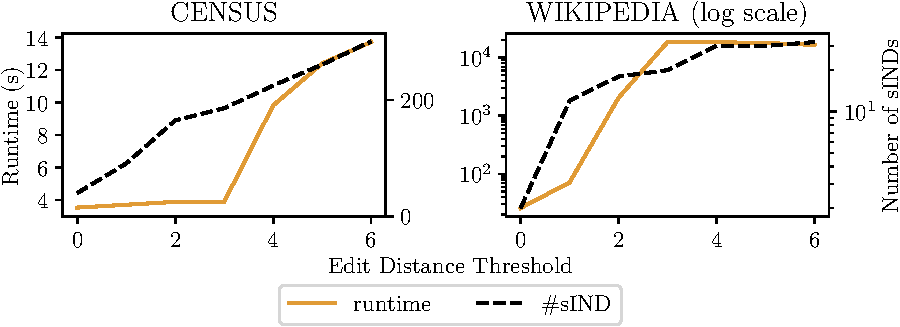
\includegraphics[width=\textwidth]{figures/ed_scaling.pdf}
        \caption{Runtime and result set size}
        \label{fig:eval:ed}
    \end{subfigure}
    \begin{subfigure}[b]{.8\textwidth}
        \centering
        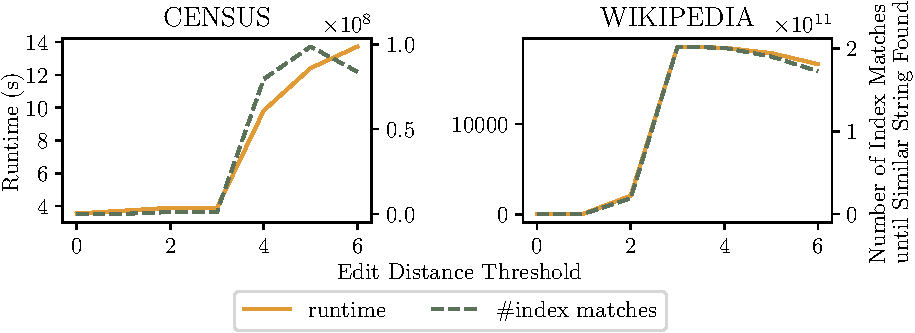
\includegraphics[width=\textwidth]{figures/ed_scaling_explanation.pdf}
        \caption{Runtime and index matches until a similar string is found}
        \label{fig:eval:ed_explanation}
    \end{subfigure}
    \caption{Edit distance threshold scaling on different datasets}
\end{figure}

Interestingly, the jump in runtime does not relate to a jump in the result set size.
To investigate the increasing runtime, we look at the number of matches in our index until a similar string was found.
Figure~\ref{fig:eval:ed_explanation} shows the runtime compared to the number of index matches.
We can observe a clear correlation.
There are two factors that influence the number of matches:
the number of dependent values that we need to validate for the candidate sINDs, and the edit distance, which influences the pruning power of the inverted index.
Since the segment length shrinks, there are more coincidental matches.
Both of these factors are dependent on the internal structure of the dataset.
For the \emph{CENSUS} dataset, we observe that there is an increase in coincidental matches for edit distance $\tau \geq 4$ because the number of index matches grows more than the number of discovered sINDs.
For $\tau = 6$, the number of index matches decreases again, because we can validate some strings earlier due to the greater edit distance.
However, the effort for each edit distance computation increases, so overall the runtime still increases.

The results for the \emph{WIKIPEDIA} dataset are on the right-hand side of Figure~\ref{fig:eval:ed}.
As before, we plot the runtime and the number of valid sINDs, here in a logarithmic scale to better show the differences in runtime.
\sawfish's runtime increases significantly for lower edit distance thresholds and reaches it peak at $\tau = 3$.
Afterward, it decreases slightly for larger edit distance thresholds, while the result set size stays almost constant.

To investigate both the stark increase and the following decrease in runtime, we regard the index matches once again.
We use linear scaling in Figure~\ref{fig:eval:ed_explanation} to better visualize the similarity of the lines.
Interestingly, the two curves have a nearly identical shape.
In contrast to the \emph{CENSUS} dataset, the early increase in the number of valid sINDs coincides with the increase in the number of index matches.
Due to the higher number of valid candidates, we have to validate more dependent values.
However, the number of index matches for $\tau = 3$ is significantly higher per dependent value than for all other edit distances.
For each dependent value, we find an average of \num{17000} index matches for $\tau = 3$, while there are only \num{8500} matches on average for $\tau = 4$.
This means that there are many index matches for $\tau = 3$ that cannot be validated.
Thus, we have to iterate the complete list of index matches for each dependent value.
In contrast, we can validate more values for $\tau = 4$, so we do not have to process all index matches.
Additionally, this explains the increase in valid sINDs for $\tau = 4$.
This trend of earlier validation continues for $\tau = 5$ and $\tau = 6$.
It also indicates that the number of coincidental matches does not increase significantly.
As explained for the \emph{CENSUS} dataset, the number of index matches decreases over-proportionally to the decrease in runtime, because each individual edit distance computation takes longer.


In conclusion, \sawfish is able to discover sINDs also for higher edit distance thresholds.
However, the runtime is dependent on the internal structure of the dataset, namely the number of valid sINDs and the number of coincidental index matches.

\paragraph{Jaccard Similarity Threshold}
We investigate the effect of different similarity thresholds $\delta$ on the \emph{TPC-H} dataset.
We focus on this dataset, because it contains strings with varying token counts; thus the difference for different thresholds is more noticeable.

Figure~\ref{fig:eval:jac_sim_scalability} shows the runtime and the result set size for different $\delta$, ranging from $0.1$ to $1.0$.
The reason for the drop in sINDs between $\delta = 0.5 \to 0.6$ is the content of the discovered sINDs.
For $\delta \leq 0.5$, we find matches between single token and two token strings that form the extra sINDs.

The runtime behavior is related to the validation characteristics, especially for values with more tokens.
For $\delta = 0.1$, for every string we need at most two matching tokens to validate the similarity, because we limit the number of tokens to 10.
For $\delta = 0.2$ and $\delta = 0.3$, we cannot validate each string so easily, but the threshold is still low.
Thus, many coincidental matches occur, which slow down the discovery process.
For $\delta \geq 0.4$, the number of coincidental matches decreases, but the validation effort for each individual value grows, because we need to find more matching tokens.
Nonetheless, the runtime converges.
This behavior is different from the edit distance case, because we discover fewer sINDs overall, but also the number of coincidental matches is lower.
\begin{figure}[ht]
    \centering
    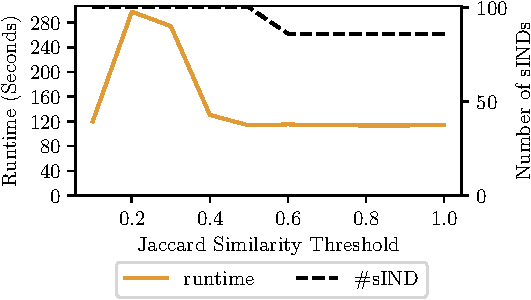
\includegraphics[width=.55\textwidth]{figures/jac_scaling.pdf}
    \caption{Jaccard similarity scalability on the \emph{TPC-H} dataset}
    \label{fig:eval:jac_sim_scalability}
\end{figure}

\subsection{Impact of Valid Dependencies}
\label{subsection:evaluation:valid_impact}
The column scalability experiment illustrated how much of the overall runtime depends on individual columns or even individual sIND candidates.
Thus, we explore this effect in more detail.
Valid dependencies contribute to the runtime especially, because we need to validate each dependent value and cannot abort early.

Figure~\ref{fig:eval:valid_dependencies} shows the runtime for each potential sIND candidate in \emph{CENSUS}, \emph{WIKIPEDIA} and \emph{TPC-H} datasets.
For clarity, we only show the results of $ED$ mode, but the findings are similar for the $JAC$ mode.
We highlight valid candidates and order the candidates by the number of distinct dependent values.
As usual, we filtered any candidates that were discarded during preprocessing.
\begin{figure}[ht]
    \centering
    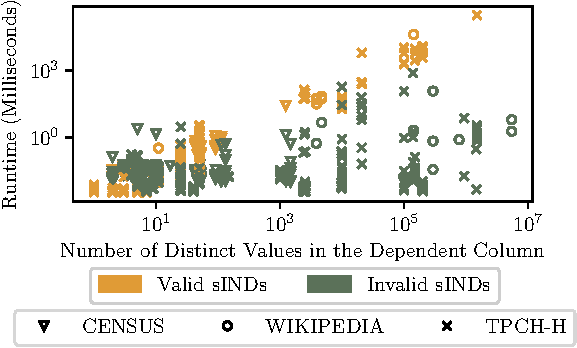
\includegraphics[width=0.6\textwidth]{figures/valid_sIND_impact.pdf}
    \caption{Difference in runtime of valid and invalid candidate validation (log-scale for both axes)}
    \label{fig:eval:valid_dependencies}
\end{figure}

We can observe two expected phenomena.
Larger dependent columns and valid dependencies need more time to validate.
The scaling behavior is more interesting.
While the runtime for valid dependencies continuously increases for larger dependent columns, the scaling is not clear for invalid dependencies.
This is because \sawfish needs to find a dependent value for which no similar referenced value exists.
Therefore, the runtime for invalid dependencies is dependent on the position of the counterexample in the dependent column and thus almost random.
This behavior can be observed especially for larger invalid dependencies, where the position differences between counterexamples are more noticeable.

\subsection{Comparison to Related Work}

The experiments in this section compare \sawfish with the baselines using all datasets.

\paragraph{Edit Distance Mode}
The following experiment compares the runtimes for an edit distance threshold $\tau = 0$. In this setting, all performance results are comparable since all algorithms discover traditional INDs.
The left-hand side of Figure~\ref{fig:eval:comparsion_ed} shows the results for all datasets, scaled per dataset to the longest running algorithm.
Interestingly, for the CENSUS dataset, our naive baseline is the fastest algorithm, while \algorithmName{Binder} needs the most time to complete the search.
Since the dataset is relatively small, the benefit of \sawfish's preprocessing does not outweigh its overhead.
Nonetheless, \sawfish is relatively close to the runtime of the baseline.

\begin{figure*}[ht]
    \centering
    \begin{subfigure}[b]{\textwidth}
        \centering
        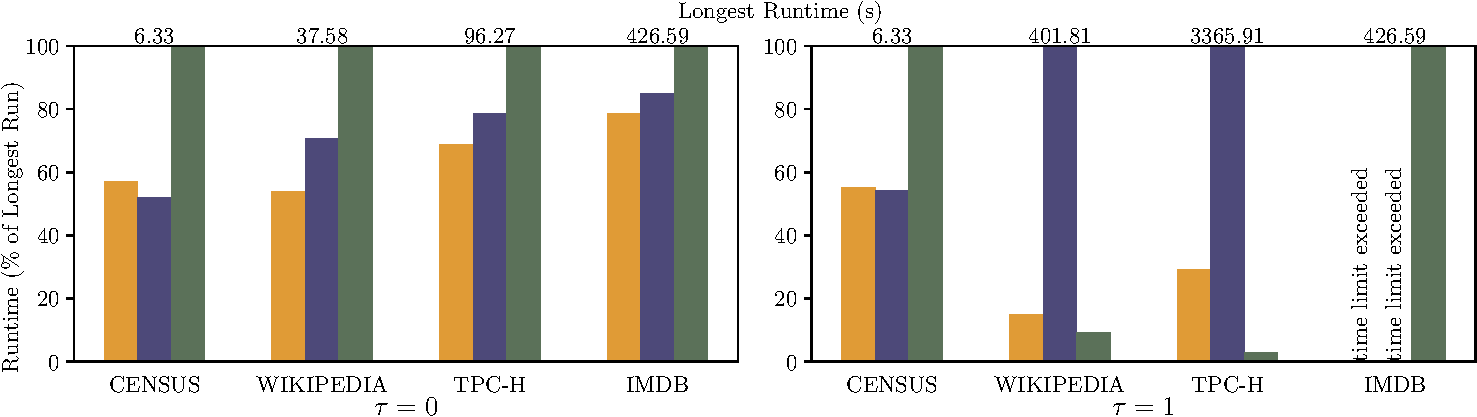
\includegraphics[width=\textwidth]{figures/competitor_ed.pdf}
        \caption{$ED$ mode}
        \label{fig:eval:comparsion_ed}
    \end{subfigure}\\
    \begin{subfigure}[b]{\textwidth}
        \centering
        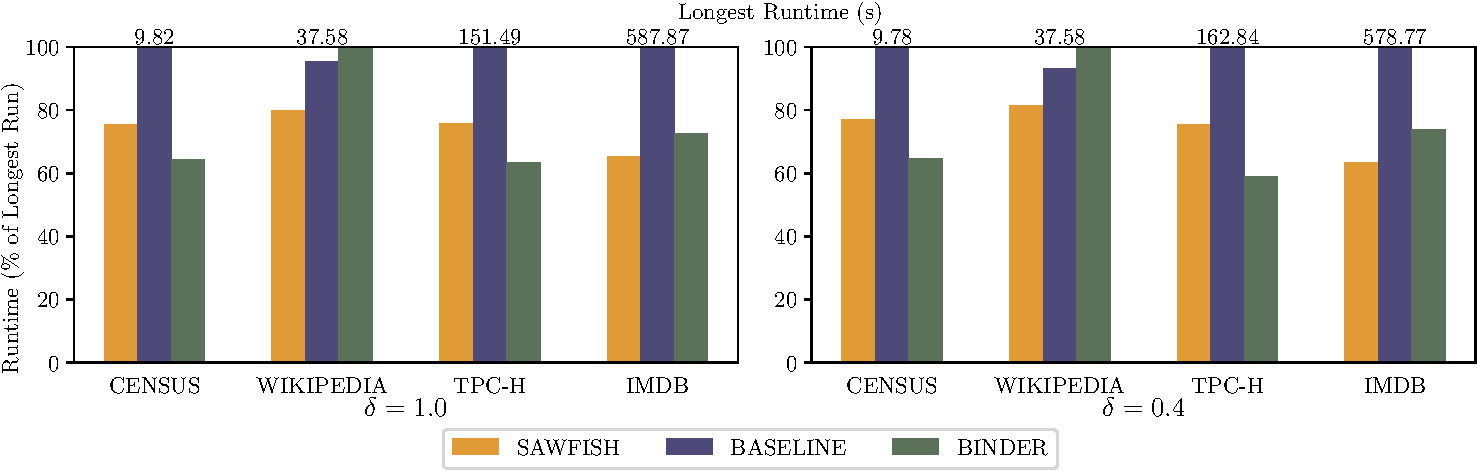
\includegraphics[width=\textwidth]{figures/competitor_jac.pdf}
        \caption{$JAC$ mode}
        \label{fig:eval:comparison_jac}
    \end{subfigure}
    \caption{Comparison of \sawfish to related work}
\end{figure*}

For the \emph{WIKIPEDIA}, the \emph{TPC-H} and the \emph{IMDB} datasets, \sawfish's preprocessing combined with the improved index access pattern improves the performance over the baseline.
\algorithmName{Binder} is the slowest in this experiment, because the two other algorithms can operate entirely in main memory if the entire dataset fits.
\algorithmName{Binder} eagerly writes every bucket to disk after preprocessing, because it anticipates larger dataset sizes.

Next, we set $\tau=1$, i.e., allow sINDs with an edit distance of up to 1 for each value.
We present them on the right-hand side of Figure~~\ref{fig:eval:comparsion_ed}.
The results for \algorithmName{Binder} remain in the figures for comparison purposes, even though \algorithmName{Binder} cannot discover such dependencies.
The result for the \emph{CENSUS} dataset is comparable in runtime to the IND discovery experiment.
However, the results for the \emph{WIKIPEDIA} dataset and the \emph{TPC-H} dataset show the superiority of \sawfish.
For the \emph{TPC-H} dataset, we observe the higher complexity of the sIND discovery compared to the IND discovery.
The runtime of \sawfish is about one third of the baseline's runtime.
This visualizes the improvements that we accomplish by modifying \algorithmName{PassJoin}'s approach.
The effect is even larger in the \emph{WIKIPEDIA} dataset:
\sawfish outperforms the baseline by a factor of around~6.5. 
\sawfish was not able to discover all sINDs for the \emph{IMDB} dataset, as it exceeded the time limit of 24~hours.
This emphasizes the difficulty of sIND discovery, because \sawfish discovered all INDs (without allowing similarity) in around 6~minutes.
We discuss ideas to improve the validation speed in Section~\ref{section:discussion}.

Our results show that \sawfish can efficiently discover sINDs for reasonably large datasets.
While the sIND discovery is a hard problem, \sawfish manages to process some datasets in a comparable time to the IND discovery.
For all larger datasets, \sawfish outperforms the baseline.

\paragraph{Jaccard Similarity Mode}
Figure~\ref{fig:eval:comparison_jac} shows the results for $\delta = 1.0$ on the left-hand side.
\algorithmName{Binder} performs best for the \emph{CENSUS} and the \emph{TPC-H} datasets, while \sawfish performs best on the other two datasets, \emph{WIKIPEDIA} and \emph{IMDB}.
Besides \algorithmName{Binder}'s algorithmic advantages, the overhead for tokenization inhibits the performance of the other two algorithms.
While \sawfish and the baseline could have found more dependencies due to the order insensitivity of the Jaccard similarity, we did not observe such effects in our dataset.
Nonetheless, they have to tokenize each value.
On the other hand, \sawfish and the baseline can once again operate entirely in main memory.
Therefore, they gain an advantage in datasets that do not create many tokens per value, e.g., \emph{WIKIPEDIA} and \emph{IMDB}.

For the next experiment, we set $\delta = 0.4$ and show the results on the right-hand side of Figure~\ref{fig:eval:comparison_jac}.
In general, the performance characteristics remain similar.
The gap between \sawfish and \algorithmName{Binder} widens a bit for the \emph{TPC-H} dataset, while it closes a bit for the \emph{WIKIPEDIA} dataset. 
For the \emph{IMDB} dataset, \sawfish and the baseline improve their runtime, because they can validate string pairs of traditional INDs earlier due to the lower threshold.

When using the Jaccard similarity, \sawfish can discover sINDs in a time that is comparable to the state-of-the-art IND discovery algorithm \algorithmName{Binder}.
We also show that \sawfish outperforms a baseline for all datasets.

\subsection{Joinability Case Study}
In this experiment, we want to investigate whether the discovered similarity inclusion dependencies can indeed indicate joinability in the presence of typos or other data errors.
Joinability means that two columns can be linked together because they contain similar data from the same domain\cite{chia2019hyperloglog}.
To investigate the performance on a more heterogeneous data source, we ran \sawfish on a subset of the \emph{2015 Web Table Corpus (WTC)}\cite{lehmberg2016corpus}.
This corpus consists of automatically crawled web tables.
While these web tables are typically smaller than traditional database tables, more web tables are usually processed simultaneously.
Our experiment uses an edit distance threshold $\tau = 1$ and the random sample of \num{10000} tables from the original source\footnote{\url{http://data.dws.informatik.uni-mannheim.de/webtables/2015-07/sample.gz}}.
However, we process only the \num{2516} relational tables in that set.
We omit numeric columns to visualize the results better.
\sawfish runs in $ED$ mode, because we find more and also more interesting results.

In total, we observe \num{1044} sINDs that consist only of strings and are not traditional INDs, i.e., the dependent column contains at least one value for which only a similar value can be found in the referenced column.

We manually annotated the sINDs to assess their genuineness.
Overall, we found 161~(15\%) meaningful sINDs, while 671~(64\%) sINDs are coincidental.
Coincidental sINDs are dependencies where the two columns contain data from different domains, but the values happen to be similar purely by chance. 
For example, we discover an sIND between the cost column of a university audiobook chapter list and the first name column of a table of probate files.
Since it is a university audiobook, all chapters are ``\data{Free}''.
Thus, the entire value set of the column contains only this value.
In turn, in the probate file table, we find the first name \data{Fred}.
The remaining 212~(20\%) sINDs are caused by errors in the header detection of the underlying dataset.

Additionally, we investigated the \emph{characteristics} of meaningful and coincidental sINDs.
For our example dataset, we observe that there are two criteria that reduce the number of coincidental sINDs significantly.
First, the maximum number of characters of any value of the dependent side is above three.
Second, the portion of dependent values that match only similarly to a value on the referenced side is below 30\%.
Given these two filters, the number of coincidental sINDs is reduced by 638 to 33~(20\%). 
The number of meaningful sINDs that fulfill these criteria is 101~(64\%).

To exemplify the discovered sINDs, we showcase some meaningful sINDs.
For example, there is an sIND between the data type column of an API description and the data type column of the input parameters of a program.
While, one column uses the uppercase versions, such as \data{Float} and \data{String}, the other column uses the lowercase versions, such as \data{float} and \data{string}.
Despite these columns obviously containing data of the same domain, they do not form a traditional IND.
Nonetheless, they could be joined to investigate usages for the same data type.

We present another example of a meaningful sIND in Table~\ref{table:eval:best_matches}.
There are multiple tables inside the sample that contain data about college athletes.
Typically, students are classified into four categories: freshman, sophomore, junior, and senior -- multiple columns contain abbreviations of these categories.
However, as the table shows, they do not match perfectly, so they do not form a traditional IND.
Interestingly, we only discover the sINDs \mbox{\emph{VCU} $\simIND{}$ \emph{CFB}} and \mbox{\emph{VCU} $\simIND{}$ \emph{NCAA}} (and their symmetric partners).
To also discover \mbox{\emph{CFB} $\simIND{}$ \emph{NCAA}}, we need to increase the edit distance threshold to~2.
Nevertheless, all of this data belongs to the same domain.
Moreover, if we want to compare students from the same category, it makes sense to join these values.
\begin{table}[h]
\centering \small
\caption{Example sINDs in the \emph{WTC} dataset}
\label{table:eval:best_matches}
\begin{tabular}{@{}lll@{}}
\toprule
VCU Football	& CFB: Tulsa Golden Hurricane	& NCAA Baseball \\
\midrule
Fr 				& FR       						& Fr.     		\\
So      		& SO                            & So.     		\\
Jr    			& JR          					& Jr.     		\\
Sr    			& SR          					& Sr.    		\\
\bottomrule
\end{tabular}
\end{table}
